\section{Koordinatensysteme}
\begin{figure}[h]
	\centering
	\begin{tikzpicture}
		% Draw axes
		\draw[->] (0,0) -- (3,0) node[right] {$x$}; % x-axis
		\draw[->] (0,0) -- (0,3) node[above] {$y$}; % y-axis
		\draw[->] (0,0) -- (-2,-2) node[below] {$z$}; %z-axis
		
		% Add grid (optional)
		%\draw[very thin, gray] (-3,-3) grid (3,3);
		
		% Add labels for the axes
		%\foreach \x in {-2,-1,1,2} % x-axis labels
		%    \draw (\x,0.1) -- (\x,-0.1) node[below] {\x};
		%\foreach \y in {-2,-1,1,2} % y-axis labels
		%    \draw (0.1,\y) -- (-0.1,\y) node[left] {\y};
		
		% Example point
		\filldraw[red] (1,2) circle (2pt) node[above] {$(x,y,z)$};
	\end{tikzpicture}
	\caption[Kartesische Koordinaten]{Das Kartesische Koordinatensystem}
	\label{fig:kart_koord}
\end{figure}

Koordinatensysteme werden zur Beschreibung physikalischer Systeme verwendet. Allgemein bekannt ist das kartesische Koordinatensystem.
Eigentlich benötigt man nur drei verschiedene Arten von Koordinaten, die kartesischen Koordinaten (Abbildung \ref{fig:kart_koord}),  die Zylinderkoordinaten (Abbildung \ref{fig:zyl_koord}) und die Kugelkoordinaten(Abbildung \ref{fig:kugel_koord}). 
Daneben gibt es auch die Polarkoordinaten. Dieses Koordinatensystem ist jedoch ein Zylinderkoordinatensystem bei welchem die z-Komponente null ist, also nur zwei Dimensionen betrachtet werden und ist daher im Folgenden unter Zylinderkoordinaten inbegriffen. 

\subsection{Zylinderkoordinaten}



\begin{figure}[h]
	\centering
\begin{tikzpicture}
	% Draw axes
	\draw[->] (0,0) -- (3,0) node[right] {$y$}; 
	\draw[->] (0,0) -- (0,3) node[above] {$z$}; 
	\draw[->] (0,0) -- (-2,-2) node[below] {$x$}; 
	
	% Draw spherical point
	\coordinate (O) at (0,0); % Origin
	\coordinate (P) at (1.5,1); % Point in spherical coordinates
	\coordinate (ProjP) at (1.5,-2); % Projection of P onto the x-y plane
	
	\draw[->, thick, red] (O) -- (1.4,0.93) node[above] {$\vec{ r }$}; % Radius vector
	\draw[dashed, gray] (P) -- (ProjP) node[below right] {}; % Projection line
	\draw[dashed, gray] (O) -- (ProjP) node[below] {}; % Projection vector in x-y plane
	
	% Add theta (polar angle)
	\draw[->, thick, blue] (0.5,0.33) arc[start angle=10, end angle=70, radius=0.7cm];
	\node[blue] at (0.2,0.5) {$\theta$};
	
	% Add phi (azimuthal angle)
	\draw[->, thick, green] (-0.5,-0.5) arc[start angle=-135, end angle=-40, radius=0.55cm];
	\node[green] at (-0.05,-0.38) {$\varphi$};
	
	% Draw labels
	%    \node[red] at (1.5,1.5) {$(r, \theta, \phi)$};
	\filldraw[red] (P) circle (2pt); % Spherical point
\end{tikzpicture}
	\caption[Kugelkoordinaten]{Die Kugelkoordinaten}
	\label{fig:kart_koord}
\end{figure}

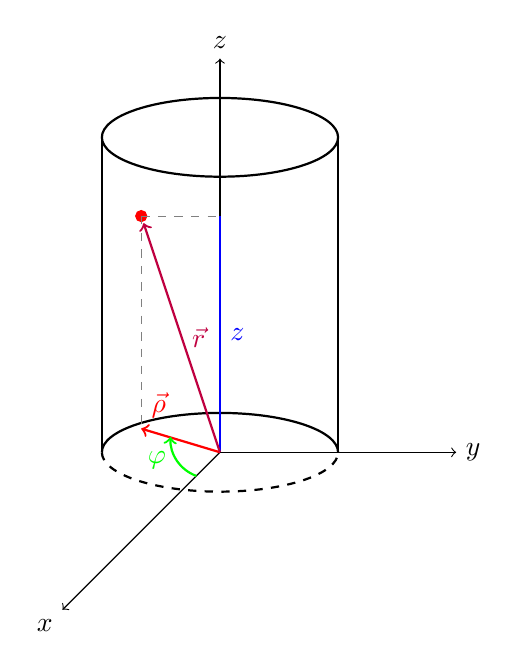
\begin{tikzpicture}
	% Draw axes
	\draw[->] (0,0) -- (3,0) node[right] {$y$}; 
	\draw[->] (0,0) -- (0,5) node[above] {$z$}; 
	\draw[->] (0,0) -- (-2,-2) node[below left] {$x$}; 
	
	% Draw the cylinder (centered on the z-axis)
	\draw[thick] (0,4) ellipse (1.5cm and 0.5cm); % Top ellipse
	\draw[thick] (-1.5,0) -- (-1.5,4); % Left side of cylinder
	\draw[thick] (1.5,0) -- (1.5,4); % Right side of cylinder
	\draw[thick, dashed] (-1.5,0) arc[start angle=180, end angle=360, x radius=1.5cm, y radius=0.5cm]; % Dashed bottom ellipse back
	\draw[thick] (-1.5,0) arc[start angle=180, end angle=0, x radius=1.5cm, y radius=0.5cm]; % Solid bottom ellipse front
	
	% Add cylindrical point
	\coordinate (O) at (0,0); % Origin
	\coordinate (P) at (-1,3); % Point in cylindrical coordinates
	\coordinate (P_for_z_vector) at (-0.97, 2.91);
	\coordinate (ProjP) at (-1,0.3); % Projection of P onto the x-y plane
	\coordinate (Projpz) at (0,3);
	
	\filldraw[red] (P) circle (2pt); % Cylindrical point
	\draw[->, thick, red] (O) -- (ProjP) node[above right] {$\vec{\rho}$}; % Radial vector
	\draw[dashed, gray] (P) -- (ProjP) node[below right] {}; % Projection line
	\draw[dashed, gray] (P) -- (Projpz) node[below right] {}; % Projection line
	\draw[blue, thick] (0,0) -- (0, 3) 	node[midway, right] {$z$};
	
	% Add azimuthal angle (phi)
	\draw[->, thick, green] (-0.3,-0.3) arc[start angle=70, end angle=-3, radius=-.5cm];
	\node[green] at (-0.8,-.1) {$\varphi$};
	
	% Add z-coordinate (height)
	\draw[->, thick, purple] (0,0) -- (P_for_z_vector) node[midway, right] {$\vec{r}$}; % Vertical vector
	
	% Draw labels
	%\node[red] at (1.2,3.2) {$(\rho, \varphi, z)$}; % Label for point P
\end{tikzpicture}